%%%%%%%%%%%%%%%%%%%%%%%%%%%%%%%%%%%%%%%%%%%%%%%%%%%%%%%%%%%%%%%%%%%%%%%%%%%%%%%%%%
\begin{frame}[fragile]\frametitle{}

\begin{center}
{\Large Word Vectors}
\end{center}
\end{frame}


%%%%%%%%%%%%%%%%%%%%%%%%%%%%%%%%%%%%%%%%%%%%%%%%%%%%%%%%%%%%%%%%%%%%%%%%%%%%%%%%%%
\begin{frame}[fragile]\frametitle{What are Word Vectors/Embeddings?}
\begin{itemize}
\item Word Embeddings are the texts converted into numbers
\item There may be different numerical representations of  same text. 
\item Many Machine Learning algorithms and almost all Deep Learning Architectures are incapable of processing strings or plain text in their raw form. 
\item They require numbers as inputs to perform any sort of job, be it classification, regression etc. in broad terms.
\item So, for the computer to be able to ''understand'' a vector representation of a word is required.
\end{itemize}
\end{frame}

%%%%%%%%%%%%%%%%%%%%%%%%%%%%%%%%%%%%%%%%%%%%%%%%%%%%%%%%%%%%%%%%%%%%%%%%%%%%%%%%%%
\begin{frame}[fragile]\frametitle{Different types of Word Vectors}
\begin{itemize}
\item (Traditional) Frequency based Embedding:
\begin{itemize}
\item One-hot
\item Count Vector
\item TF-IDF Vector
\item Co-Occurrence Vector
\end{itemize}
\item (Modern) Prediction based Embedding:
\begin{itemize}
\item Word2vec  (Google)
\item Global Vector Representations (GloVe)   (Stanford)
\end{itemize}
\end{itemize}
\end{frame}


%%%%%%%%%%%%%%%%%%%%%%%%%%%%%%%%%%%%%%%%%%%%%%%%%%%%%%%%%%%%%%%%%%%%%%%%%%%%%%%%%%
\begin{frame}[fragile]\frametitle{One Hot}
\begin{center}
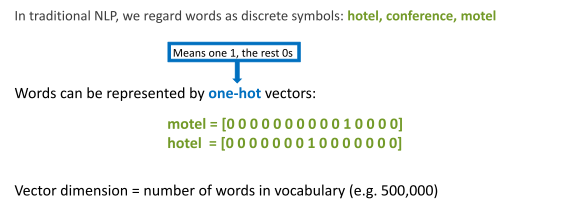
\includegraphics[width=\linewidth,keepaspectratio]{emb4}
\end{center}

{\tiny (Ref: Word Embeddings - Elena Voita, Yandex Research}
\end{frame}


%%%%%%%%%%%%%%%%%%%%%%%%%%%%%%%%%%%%%%%%%%%%%%%%%%%%%%%%%%%%%%%%%%%%%%%%%%%%%%%%%%
\begin{frame}[fragile]\frametitle{One Hot: Problem}
\begin{center}
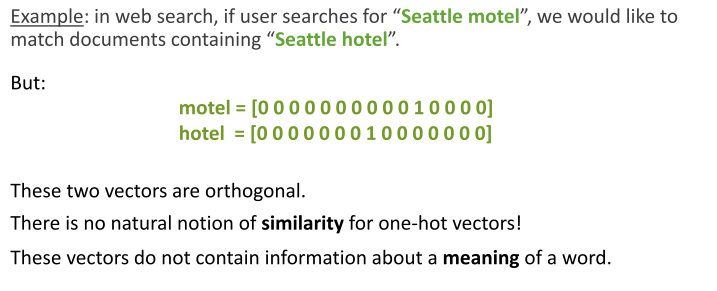
\includegraphics[width=\linewidth,keepaspectratio]{emb5}
\end{center}

{\tiny (Ref: Word Embeddings - Elena Voita, Yandex Research)}
\end{frame}

%%%%%%%%%%%%%%%%%%%%%%%%%%%%%%%%%%%%%%%%%%%%%%%%%%%%%%%%%%%%%%%%%%%%%%%%%%%%%%%%%%
\begin{frame}[fragile]\frametitle{One Hot: Example}
One-hot:  Suppose our vocabulary has only five words: King, Queen, Man, Woman, and Child. We could encode the word `Queen' as:
\begin{center}
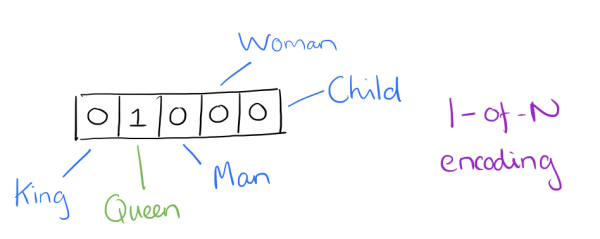
\includegraphics[width=0.8\linewidth,keepaspectratio]{word40}
\end{center}
No meaningful comparison possible. We will look at some vectorization schemes that can capture ``meaning'', somewhat.
\end{frame}


%%%%%%%%%%%%%%%%%%%%%%%%%%%%%%%%%%%%%%%%%%%%%%%%%%%%%%%%%%%%%%%%%%%%%%%%%%%%%%%%%%
\begin{frame}[fragile]\frametitle{Count Vector}
\begin{itemize}
\item Corpus:
\begin{itemize}
\item D1: He is a lazy boy. She is also lazy.
\item D2: Neeraj is a lazy person.
\end{itemize}
\item Dictionary is a list of unique tokens(words) =['He','She','lazy','boy','Neeraj','person'] 
\item Count Matrix:
\begin{center}
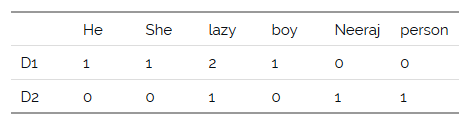
\includegraphics[width=\linewidth,keepaspectratio]{word29}
\end{center}
\end{itemize}
\end{frame}

%%%%%%%%%%%%%%%%%%%%%%%%%%%%%%%%%%%%%%%%%%%%%%%%%%%%%%%%%%%%%%%%%%%%%%%%%%%%%%%%%%
\begin{frame}[fragile]\frametitle{Count Vector}
\begin{center}
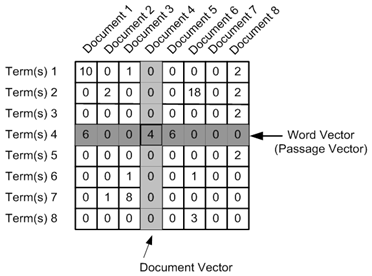
\includegraphics[width=0.8\linewidth,keepaspectratio]{word30}
\end{center}
\end{frame}

%%%%%%%%%%%%%%%%%%%%%%%%%%%%%%%%%%%%%%%%%%%%%%%%%%%%%%%%%%%%%%%%%%%%%%%%%%%%%%%%%%
\begin{frame}[fragile]\frametitle{TF-IDF vectorization}
\begin{itemize}
\item It takes into account not just the occurrence of a word in a single document but in the entire corpus.
\item Down weight the common words occurring in almost all documents and give more importance to words that appear in a subset of documents.
\item Corpus:
\begin{center}
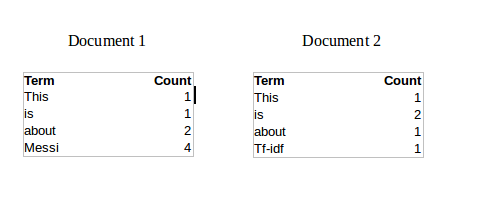
\includegraphics[width=0.8\linewidth,keepaspectratio]{word31}
\end{center}
\end{itemize}
\end{frame}

%%%%%%%%%%%%%%%%%%%%%%%%%%%%%%%%%%%%%%%%%%%%%%%%%%%%%%%%%%%%%%%%%%%%%%%%%%%%%%%%%%
\begin{frame}[fragile]\frametitle{TF-IDF vectorization}
\begin{itemize}
\item TF = (Number of times term t appears in a document)/(Number of terms in the document)
\item So, TF(This,Document1) = 1/8  and TF(This, Document2)=1/5
\item IDF = log(N/n), where, N is the number of documents and n is the number of documents a term t has appeared in.
\item So, IDF(This) = log(2/2) = 0.
\item TFIDF = TF*IDF
\item Dictionary is made of a list of unique tokens(words) 
\item Similar to Count Matrix, TFIDF matrix is made with TFIDF values in it.
\end{itemize}
\end{frame}


%%%%%%%%%%%%%%%%%%%%%%%%%%%%%%%%%%%%%%%%%%%%%%%%%%%%%%%%%%%%%%%%%%%%%%%%%%%%%%%%%%
\begin{frame}[fragile]\frametitle{Co-Occurrence Matrix}
\begin{itemize}
\item Co-occurrence ' For a given corpus, the co-occurrence of a pair of words say w1 and w2 is the number of times they have appeared together in a Context Window.
\item Context Window ' Context window is specified by a number and the direction. So what does a context window of 2 (around) means?
\begin{center}
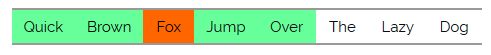
\includegraphics[width=0.6\linewidth,keepaspectratio]{word32}
\end{center}
\item For Corpus ='' He is not lazy. He is intelligent. He is smart.''
\end{itemize}
\begin{center}
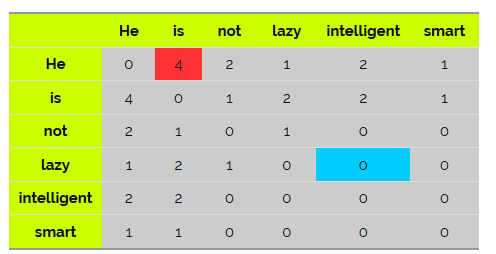
\includegraphics[width=0.5\linewidth,keepaspectratio]{word33}
\end{center}
\end{frame}

%%%%%%%%%%%%%%%%%%%%%%%%%%%%%%%%%%%%%%%%%%%%%%%%%%%%%%%%%%%%%%%%%%%%%%%%%%%%%%%%%%
\begin{frame}[fragile]\frametitle{Co-Occurrence Matrix}
Red box- It is the number of times 'He' and 'is' have appeared in the context window 2 and it can be seen that the count turns out to be 4. 
\begin{center}
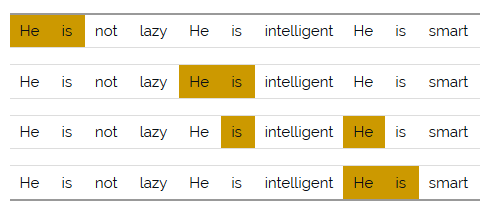
\includegraphics[width=0.5\linewidth,keepaspectratio]{word34}
\end{center}
While the word 'lazy' has never appeared with'intelligent' in the context window and therefore has been assigned 0 in the blue box.
\end{frame}



%%%%%%%%%%%%%%%%%%%%%%%%%%%%%%%%%%%%%%%%%%%%%%%%%%%%%%%%%%%%%%%%%%%%%%%%%%%%%%%%%%
\begin{frame}[fragile]\frametitle{Good Vector Representation}
\begin{itemize}
\item To have ''Semantic'' (meaning-wise) representation, the Similar words should be close to each other in the hyper dimensional space.
\item Non-similar words should be far apart from each other in the hyper dimensional space.
\end{itemize}
\end{frame}

%%%%%%%%%%%%%%%%%%%%%%%%%%%%%%%%%%%%%%%%%%%%%%%%%%%%%%%%%%%%%%%%%%%%%%%%%%%%%%%%%%
\begin{frame}[fragile]\frametitle{Good Vector Representation}
\begin{itemize}
\item Traditional One Hot Encoding:
	\begin{itemize}
	\item Apple = [1, 0, 0]
	\item Orange = [0, 1, 0]
	\item Plane = [0, 0, 1]
	\end{itemize}
\begin{center}
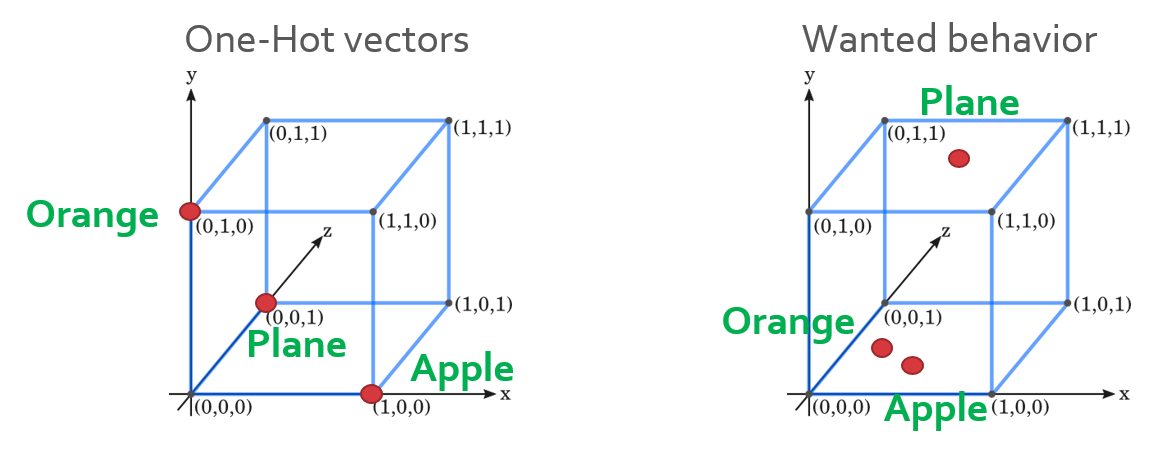
\includegraphics[width=0.6\linewidth,keepaspectratio]{word23_1}
\end{center}
\item Very few cells participate in the representation.
\end{itemize}
\end{frame}


%%%%%%%%%%%%%%%%%%%%%%%%%%%%%%%%%%%%%%%%%%%%%%%%%%%%%%%%%%%%%%%%%%%%%%%%%%%%%%%%%%
\begin{frame}[fragile]\frametitle{But, What is ``meaning''?}
What is ``bardiwac''?

Anyone?
\end{frame}

%%%%%%%%%%%%%%%%%%%%%%%%%%%%%%%%%%%%%%%%%%%%%%%%%%%%%%%%%%%%%%%%%%%%%%%%%%%%%%%%%%
\begin{frame}[fragile]\frametitle{Lets try again, with examples}
What is ``bardiwac''?

\begin{itemize}
\item He handed her a glass of \underline{bardiwac}. 
\item Beef dishes are made to complement the \underline{bardiwac}.
\item Nigel staggered to his feet, face flushed from too much
\underline{bardiwac}. 
\item Malbec, one of the lesser-known \underline{bardiwac} grapes,
responds well to Australia’s sunshine. 
\item I dined off bread and cheese and this excellent \underline{bardiwac}. 
\item The drinks were delicious: blood-red \underline{bardiwac} as well as 
light, sweet Rhenish. 
\end{itemize}

Now, anyone?
\end{frame}

%%%%%%%%%%%%%%%%%%%%%%%%%%%%%%%%%%%%%%%%%%%%%%%%%%%%%%%%%%%%%%%%%%%%%%%%%%%%%%%%%%
\begin{frame}[fragile]\frametitle{At least one can guess now}
What is ``bardiwac''?

``Bardiwac is a red 
alcoholic beverage 
made from grapes ''

Context helps \ldots
\end{frame}

%%%%%%%%%%%%%%%%%%%%%%%%%%%%%%%%%%%%%%%%%%%%%%%%%%%%%%%%%%%%%%%%%%%%%%%%%%%%%%%%%%
\begin{frame}[fragile]\frametitle{Distributed Semantics/Meaning}
\begin{itemize}
\item  A bottle of \underline{bardiwac} is on the table. 
\item  Everybody likes \underline{bardiwac}.
\item  Don’t have \underline{bardiwac} before you drive. 
\item  We make \underline{bardiwac}  out of corn. 

\end{itemize}
\end{frame}

%%%%%%%%%%%%%%%%%%%%%%%%%%%%%%%%%%%%%%%%%%%%%%%%%%%%%%%%%%%%%%%%%%%%%%%%%%%%%%%%%%
\begin{frame}[fragile]\frametitle{Distributed Semantics/Meaning}
\begin{itemize}
\item  A bottle of \underline{xxxxxxxx} is on the table. 
\item  Everybody likes \underline{xxxxxxxx}.
\item  Don’t have \underline{xxxxxxxx} before you drive. 
\item  We make \underline{xxxxxxxx}  out of corn. 

\end{itemize}

What other words fit into these places? 

Won't they be similar to bardiwac?
\end{frame}

%%%%%%%%%%%%%%%%%%%%%%%%%%%%%%%%%%%%%%%%%%%%%%%%%%%%%%%%%%%%%%%%%%%%%%%%%%%%%%%%%%
\begin{frame}[fragile]\frametitle{Distributed Semantics/Meaning}
\begin{center}
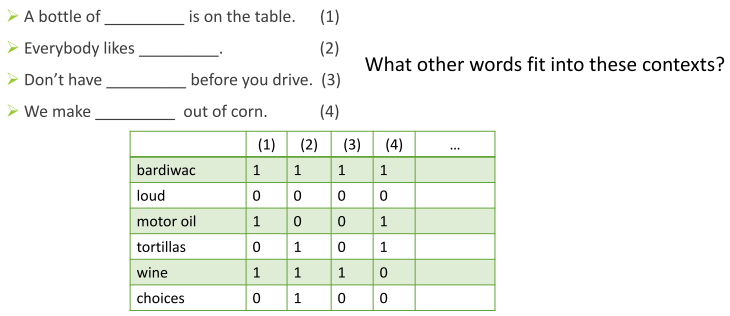
\includegraphics[width=\linewidth,keepaspectratio]{emb6}
\end{center}

{\tiny (Ref: Word Embeddings - Elena Voita, Yandex Research}
\end{frame}



%%%%%%%%%%%%%%%%%%%%%%%%%%%%%%%%%%%%%%%%%%%%%%%%%%%%%%%%%%%%%%%%%%%%%%%%%%%%%%%%%%
\begin{frame}[fragile]\frametitle{Distributed Semantics/Meaning}
Closer ones are \ldots

\begin{center}
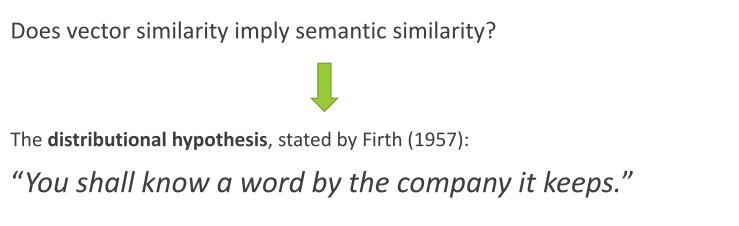
\includegraphics[width=0.8\linewidth,keepaspectratio]{emb8}
\end{center}

{\tiny (Ref: Word Embeddings - Elena Voita, Yandex Research)}
\end{frame}

%%%%%%%%%%%%%%%%%%%%%%%%%%%%%%%%%%%%%%%%%%%%%%%%%%%%%%%%%%%%%%%%%%%%%%%%%%%%%%%%%%
\begin{frame}[fragile]\frametitle{Distributed Semantics/Meaning}
Closer ones are \ldots

\begin{center}
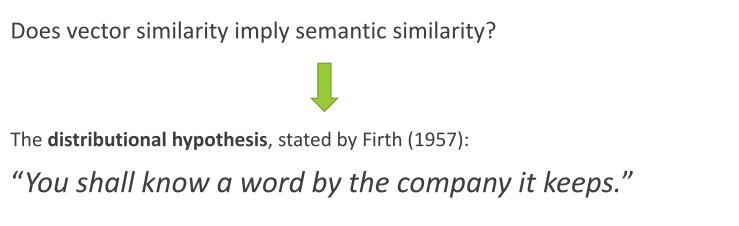
\includegraphics[width=0.8\linewidth,keepaspectratio]{emb8}
\end{center}

{\tiny (Ref: Word Embeddings - Elena Voita, Yandex Research}
\end{frame}

%%%%%%%%%%%%%%%%%%%%%%%%%%%%%%%%%%%%%%%%%%%%%%%%%%%%%%%%%%%%%%%%%%%%%%%%%%%%%%%%%%
\begin{frame}[fragile]\frametitle{Distributed Semantics/Meaning}
Idea of Co-occurance counts \ldots

\begin{center}
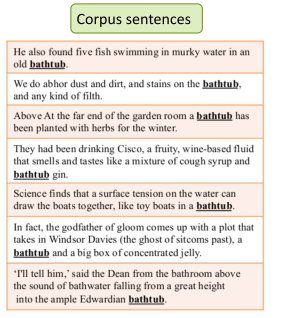
\includegraphics[width=0.4\linewidth,keepaspectratio]{emb9}
\end{center}

{\tiny (Ref: Word Embeddings - Elena Voita, Yandex Research)}
\end{frame}

%%%%%%%%%%%%%%%%%%%%%%%%%%%%%%%%%%%%%%%%%%%%%%%%%%%%%%%%%%%%%%%%%%%%%%%%%%%%%%%%%%
\begin{frame}[fragile]\frametitle{Distributed Semantics/Meaning}
Calculate Co-occurrences for the context word, that itself becomes its own representation!!!

\begin{center}
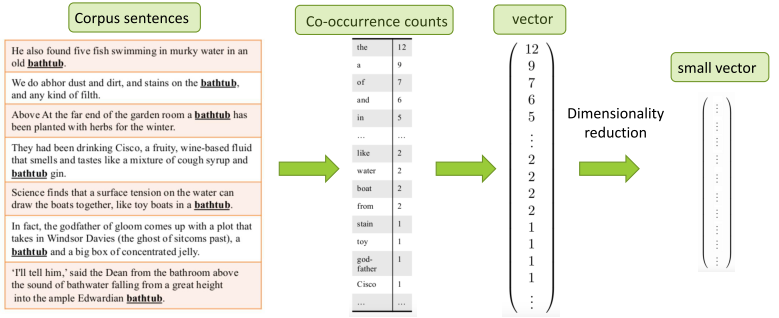
\includegraphics[width=\linewidth,keepaspectratio]{emb10}
\end{center}

{\tiny (Ref: Word Embeddings - Elena Voita, Yandex Research)}
\end{frame}



%%%%%%%%%%%%%%%%%%%%%%%%%%%%%%%%%%%%%%%%%%%%%%%%%%%%%%%%%%%%%%%%%%%%%%%%%%%%%%%%%%
\begin{frame}[fragile]\frametitle{Examples}
\begin{center}
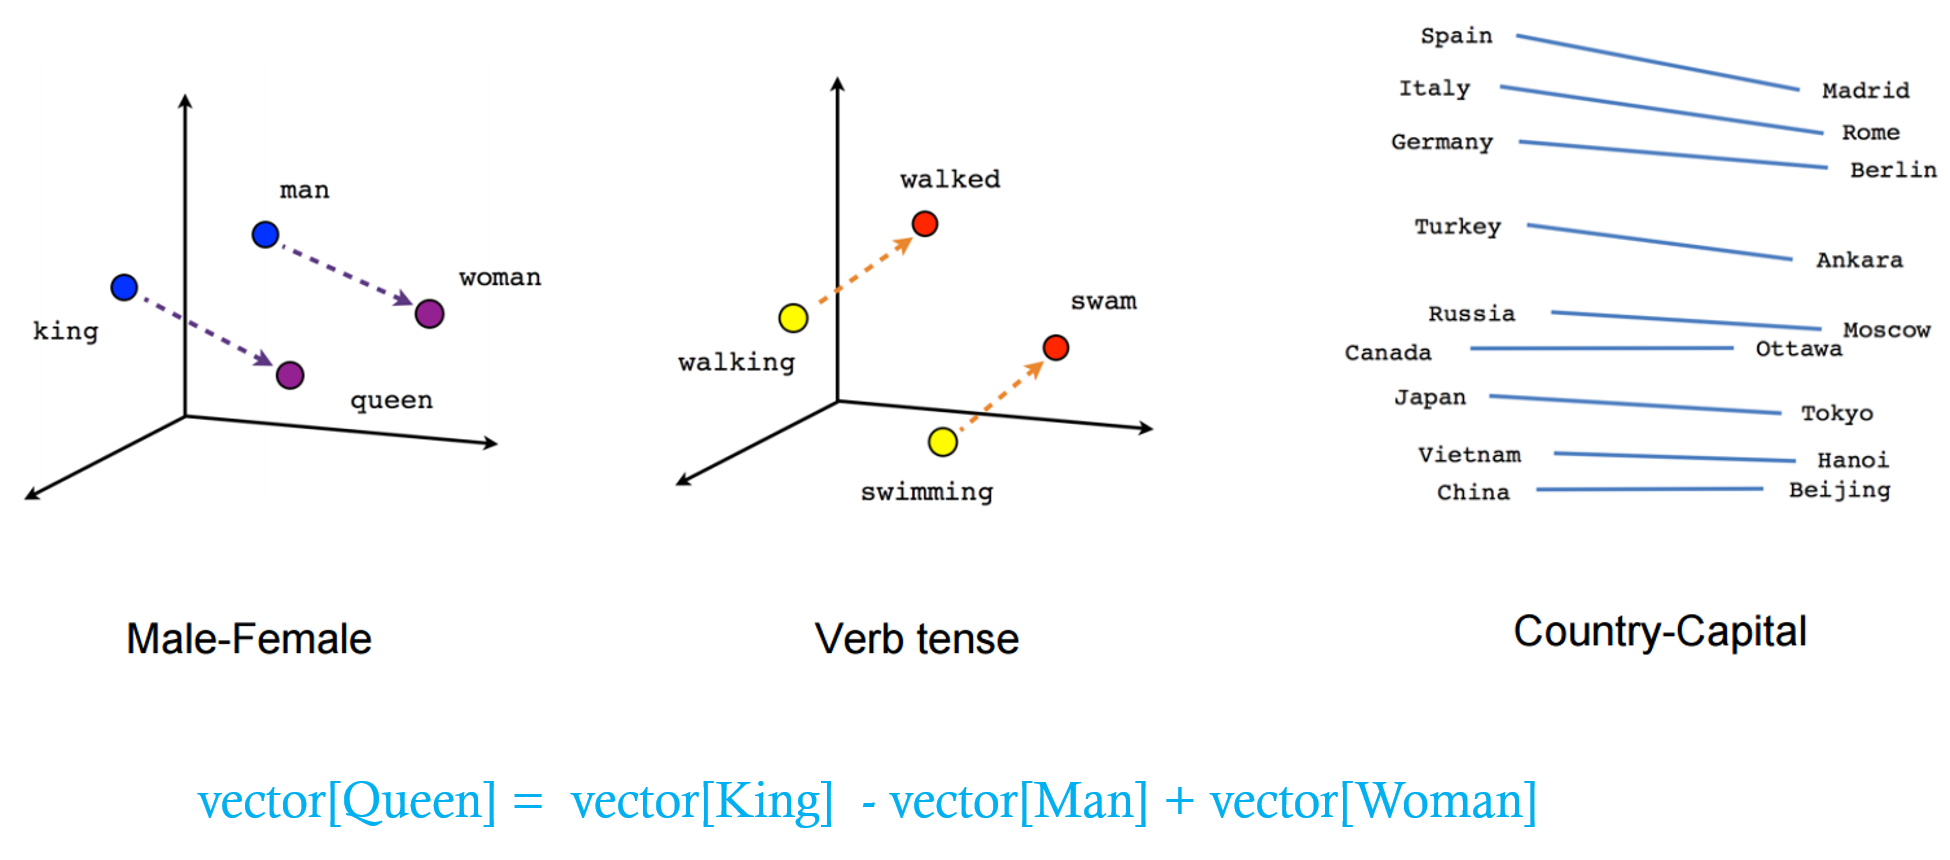
\includegraphics[width=\linewidth,keepaspectratio]{word12}
\end{center}
\end{frame}

%%%%%%%%%%%%%%%%%%%%%%%%%%%%%%%%%%%%%%%%%%%%%%%%%%%%%%%%%%%%%%%%%%%%%%%%%%%%%%%%%%
\begin{frame}[fragile]\frametitle{Building these magical vectors }
\begin{itemize}
\item How do we actually build these super-intelligent vectors, that seem to have such magical powers?
\item How to find a word's friends?
\item We will discuss the most famous methods to build such lower-dimension vector representations for words based on their context
\begin{itemize}
\item Co-occurrence Matrix with SVD
\item word2vec  (Google)
\item Global Vector Representations (GloVe)   (Stanford)
\end{itemize}
\end{itemize}
\end{frame}

% %%%%%%%%%%%%%%%%%%%%%%%%%%%%%%%%%%%%%%%%%%%%%%%%%%%%%%%%%%%%%%%%%%%%%%%%%%%%%%%%%%
% \begin{frame}[fragile]\frametitle{Co-occurrence Matrix}
% Co-occurrence Matrix with Singular Value Decomposition:
% \begin{center}
% 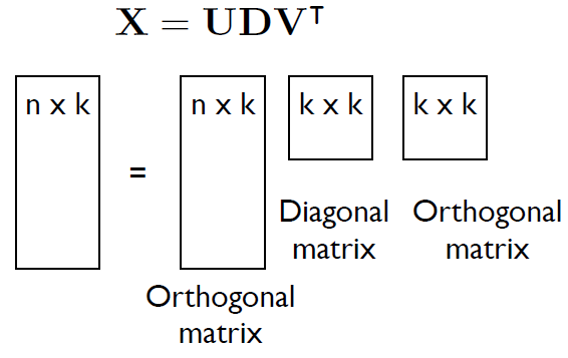
\includegraphics[width=0.5\linewidth,keepaspectratio]{word16}
% \end{center}
% \end{frame}


% %%%%%%%%%%%%%%%%%%%%%%%%%%%%%%%%%%%%%%%%%%%%%%%%%%%%%%%%%%%%%%%%%%%%%%%%%%%%%%%%%%
% \begin{frame}[fragile]\frametitle{Building a co-occurrence matrix}
% \begin{lstlisting}
% Corpus =  {``I like deep learning''
	    % ``I like NLP''
	    % ``I enjoy flying''} 
% \end{lstlisting}
% \begin{center}
% 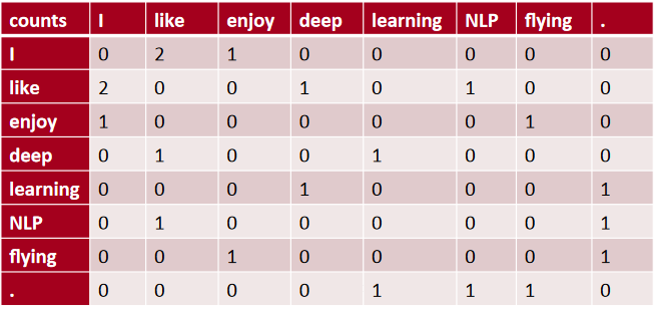
\includegraphics[width=\linewidth,keepaspectratio]{word17}
% \end{center}
% Context =  previous word and next word
% \end{frame}

% %%%%%%%%%%%%%%%%%%%%%%%%%%%%%%%%%%%%%%%%%%%%%%%%%%%%%%%%%%%%%%%%%%%%%%%%%%%%%%%%%%
% \begin{frame}[fragile]\frametitle{Dimension Reduction using Singular Value Decomposition}
% \begin{center}
% 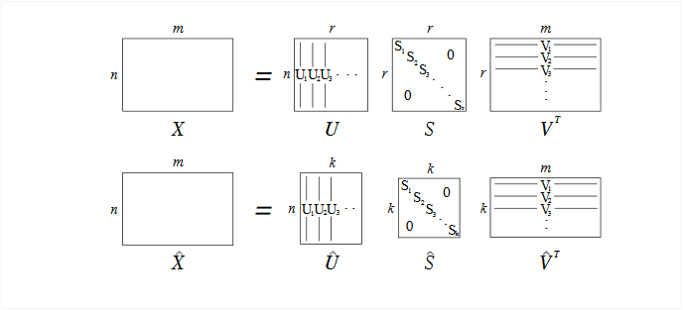
\includegraphics[width=\linewidth,keepaspectratio]{word18}
% \end{center}
% \end{frame}

% %%%%%%%%%%%%%%%%%%%%%%%%%%%%%%%%%%%%%%%%%%%%%%%%%%%%%%%%%%%%%%%%%%%%%%%%%%%%%%%%%%
% \begin{frame}[fragile]\frametitle{Singular Value Decomposition}
% \begin{center}
% 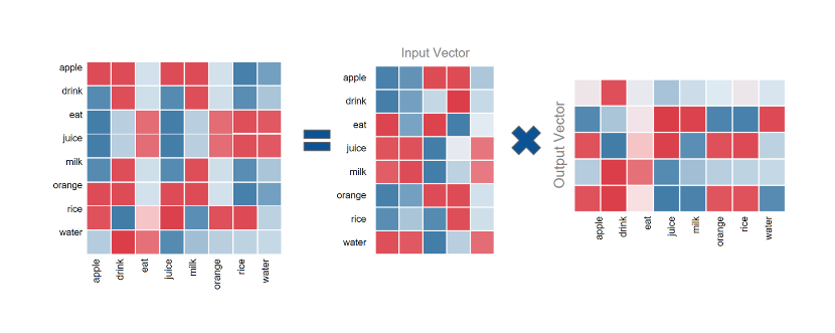
\includegraphics[width=\linewidth,keepaspectratio]{word19}
% \end{center}
% The problem with this method, is that we may end up with matrices having billions of rows and columns, which makes SVD computationally restrictive.

% \end{frame}




%%%%%%%%%%%%%%%%%%%%%%%%%%%%%%%%%%%%%%%%%%%%%%%%%%%%%%%%%%%%%%%%%%%%%%%%%%%%%%%%%
\begin{frame}[fragile]\frametitle{Language Model }
\begin{itemize}
\item A good statistical model for NLP is the conditional probability of the next word w given its previous ones
\item Takes advantage of both word order, and the fact that temporally closer words have a stronger dependency.
\item Continues Bag - of - Words (CBOW): predicts a word given its context (bidirectional).
\item Skip - Gram: predicts the context given a word (bidirectional).
\end{itemize}
\begin{center}
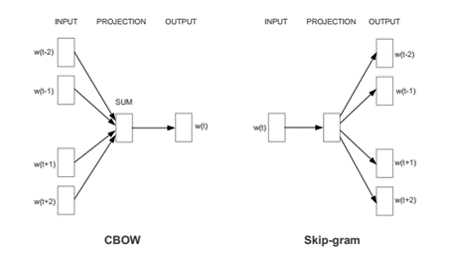
\includegraphics[width=0.5\linewidth,keepaspectratio]{word25}
\end{center}
(Ref: Distributed Representations of Words and Phrases and their Compositionality. Mikolov at al., 2013)
\end{frame}

% %%%%%%%%%%%%%%%%%%%%%%%%%%%%%%%%%%%%%%%%%%%%%%%%%%%%%%%%%%%%%%%%%%%%%%%%%%%%%%%%%%
% \begin{frame}[fragile]\frametitle{Word2Vec}
% \begin{center}
% 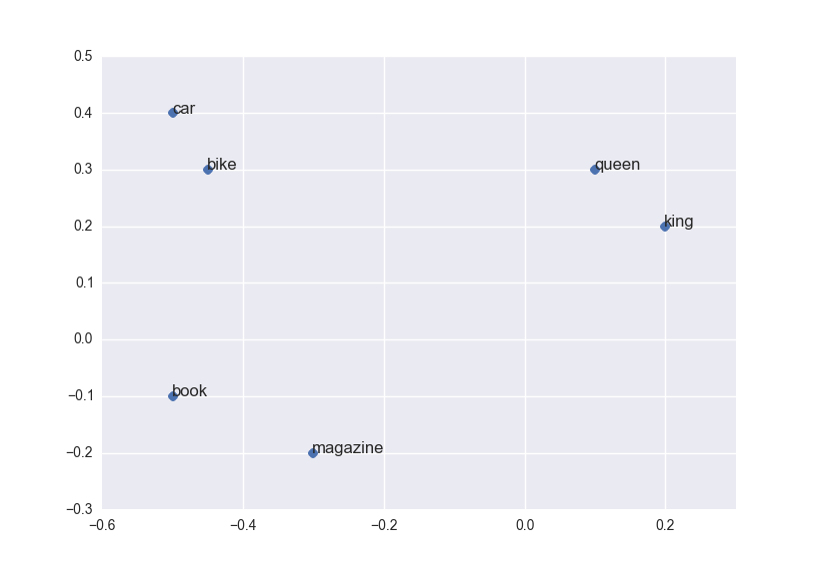
\includegraphics[width=\linewidth,keepaspectratio]{word20}
% \end{center}
% \end{frame}

% %%%%%%%%%%%%%%%%%%%%%%%%%%%%%%%%%%%%%%%%%%%%%%%%%%%%%%%%%%%%%%%%%%%%%%%%%%%%%%%%%
% \begin{frame}[fragile]\frametitle{Word2Vec Architecture}
% \begin{center}
% 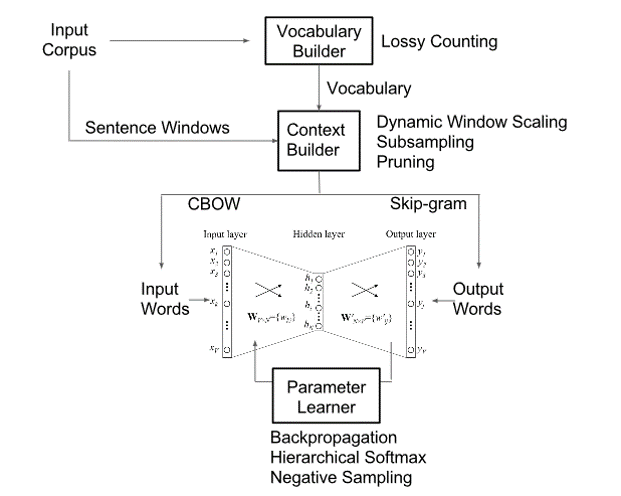
\includegraphics[width=0.8\linewidth,keepaspectratio]{word21}
% \end{center}
% \end{frame}


%%%%%%%%%%%%%%%%%%%%%%%%%%%%%%%%%%%%%%%%%%%%%%%%%%%%%%%%%%%%%%%%%%%%%%%%%%%%%%%%%
\begin{frame}[fragile]\frametitle{Context windows}
\begin{itemize}
\item Context can be anything - a surrounding n-gram, a randomly sampled set of words from a fixed size window around the word
\item For example, assume context is defined as the word following a word. $context(w_i) = w_{i+1}$
\item Corpus :  I ate the cat
\item Training Set  : $I|ate,  ate|the ,  the|cat, cat|. $
\end{itemize}
\end{frame}


%%%%%%%%%%%%%%%%%%%%%%%%%%%%%%%%%%%%%%%%%%%%%%%%%%%%%%%%%%%%%%%%%%%%%%%%%%%%%%%%%%
\begin{frame}[fragile]\frametitle{Google's Word2Vec}
\begin{center}
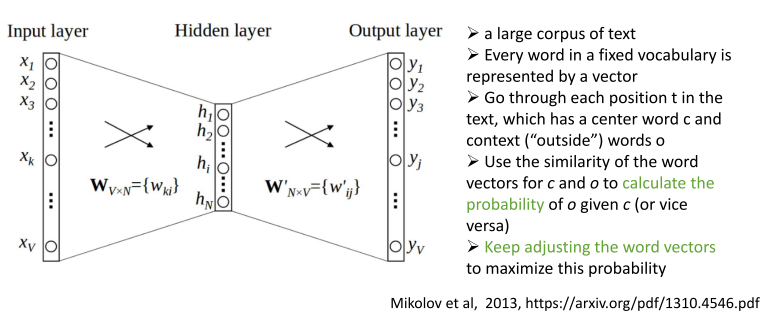
\includegraphics[width=\linewidth,keepaspectratio]{emb11}
\end{center}

{\tiny (Ref: Word Embeddings - Elena Voita, Yandex Research)}
\end{frame}

%%%%%%%%%%%%%%%%%%%%%%%%%%%%%%%%%%%%%%%%%%%%%%%%%%%%%%%%%%%%%%%%%%%%%%%%%%%%%%%%%%
\begin{frame}[fragile]\frametitle{Word2Vec Procedure}
\begin{center}
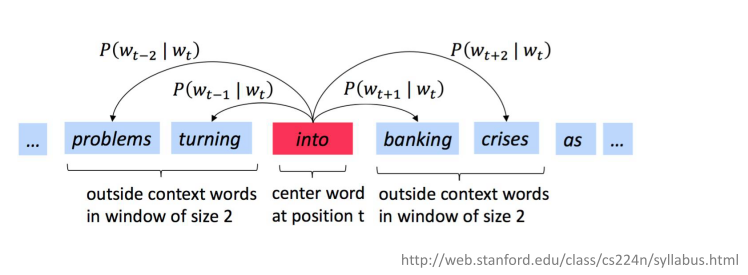
\includegraphics[width=\linewidth,keepaspectratio]{emb12}
\end{center}

{\tiny (Ref: Word Embeddings - Elena Voita, Yandex Research)}
\end{frame}

%%%%%%%%%%%%%%%%%%%%%%%%%%%%%%%%%%%%%%%%%%%%%%%%%%%%%%%%%%%%%%%%%%%%%%%%%%%%%%%%%%
\begin{frame}[fragile]\frametitle{Word2Vec Optimization}
\begin{center}
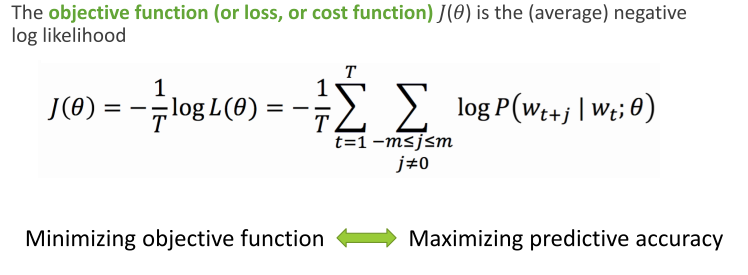
\includegraphics[width=\linewidth,keepaspectratio]{emb13}
\end{center}

$\theta$s are all the weights in the neural network.

{\tiny (Ref: Word Embeddings - Elena Voita, Yandex Research)}
\end{frame}


% %%%%%%%%%%%%%%%%%%%%%%%%%%%%%%%%%%%%%%%%%%%%%%%%%%%%%%%%%%%%%%%%%%%%%%%%%%%%%%%%%%
% \begin{frame}[fragile]\frametitle{Intuitive Idea}
% \begin{center}
% 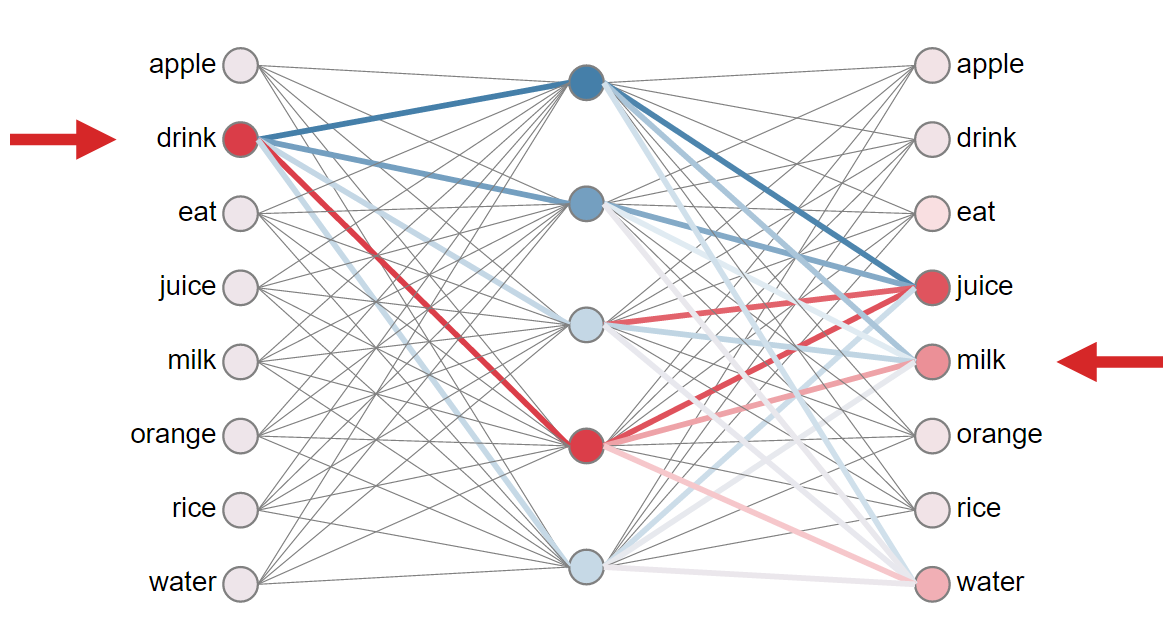
\includegraphics[width=\linewidth,keepaspectratio]{word22}
% \end{center}
% \end{frame}


%%%%%%%%%%%%%%%%%%%%%%%%%%%%%%%%%%%%%%%%%%%%%%%%%%%%%%%%%%%%%%%%%%%%%%%%%%%%%%%%%%
\begin{frame}[fragile]\frametitle{Word2Vec: CBOW}
\begin{center}
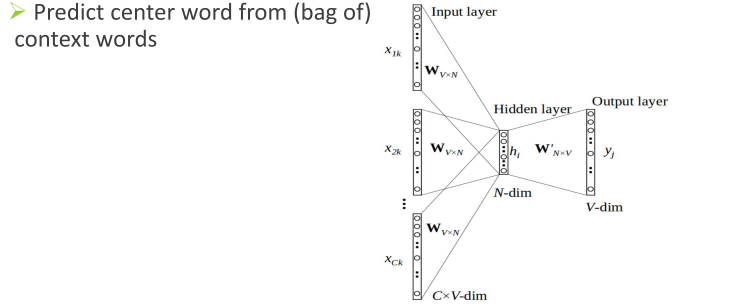
\includegraphics[width=\linewidth,keepaspectratio]{emb14}
\end{center}

{\tiny (Ref: Word Embeddings - Elena Voita, Yandex Research)}
\end{frame}


%%%%%%%%%%%%%%%%%%%%%%%%%%%%%%%%%%%%%%%%%%%%%%%%%%%%%%%%%%%%%%%%%%%%%%%%%%%%%%%%%
\begin{frame}[fragile]\frametitle{CBOW (Continuous Bag of words)}
\begin{itemize}
\item Predicts the probability of a word given a context. 
\item A context may be a single word or a group of words. 
\item  Corpus =``Hey, this is sample corpus using only one context word.''
\item training set with window 1
\item The input layer and the target, both are one- hot encoded of size [1 X V]. Here V=10 in the above example.
\item There are two sets of weights. one is between the input and the hidden layer and second between hidden and output layer.
\item N is the number of dimensions, say 4.
\end{itemize}
\begin{center}
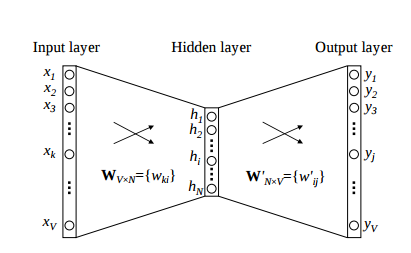
\includegraphics[width=0.3\linewidth,keepaspectratio]{word35}
\end{center}
\end{frame}

%%%%%%%%%%%%%%%%%%%%%%%%%%%%%%%%%%%%%%%%%%%%%%%%%%%%%%%%%%%%%%%%%%%%%%%%%%%%%%%%%
\begin{frame}[fragile]\frametitle{CBOW (Continuous Bag of words)}
\begin{itemize}
\item The context words form the input layer. 
\item Each word is encoded in one-hot form.
\item There is a single hidden layer and an output layer.
\end{itemize}
\begin{center}
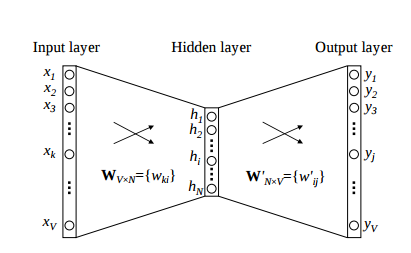
\includegraphics[width=0.5\linewidth,keepaspectratio]{word35}
\end{center}

\end{frame}

%%%%%%%%%%%%%%%%%%%%%%%%%%%%%%%%%%%%%%%%%%%%%%%%%%%%%%%%%%%%%%%%%%%%%%%%%%%%%%%%%
\begin{frame}[fragile]\frametitle{CBOW (Continuous Bag of words)}

\begin{center}
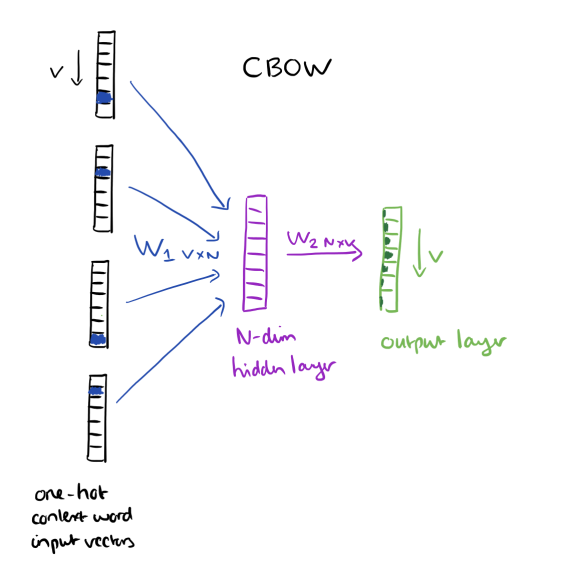
\includegraphics[width=0.5\linewidth,keepaspectratio]{word49}
\end{center}
\begin{itemize}
\item $V^T(1xv) \times W_1(vxN) = Hidden(1xN)$
\item $Hidden(1xN)  \times W_2(Nxv) = Output(1xv)$
\end{itemize}
\end{frame}

%%%%%%%%%%%%%%%%%%%%%%%%%%%%%%%%%%%%%%%%%%%%%%%%%%%%%%%%%%%%%%%%%%%%%%%%%%%%%%%%%
\begin{frame}[fragile]\frametitle{CBOW (Continuous Bag of words)}
\begin{itemize}
\item The training objective is to maximize the conditional probability of observing the actual output word (the focus word) given the input context words, with regard to the weights. 
\item Since our input vectors are one-hot, multiplying an input vector by the weight matrix W1 amounts to simply selecting a row from W1.

\begin{center}
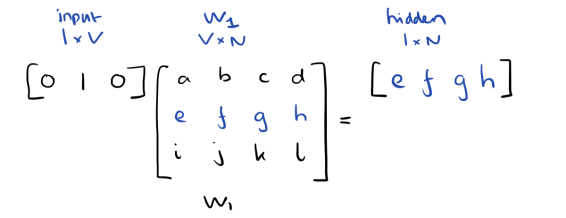
\includegraphics[width=0.8\linewidth,keepaspectratio]{word50}
\end{center}
\end{itemize}
\end{frame}

%%%%%%%%%%%%%%%%%%%%%%%%%%%%%%%%%%%%%%%%%%%%%%%%%%%%%%%%%%%%%%%%%%%%%%%%%%%%%%%%%
\begin{frame}[fragile]\frametitle{CBOW (Continuous Bag of words)}
\begin{itemize}
\item Lets say V=8, N=3 
\item Means that $W_1$ and $W_2$ will be 8 x 3 and 3x 8 matrices,

\begin{center}
$W_1$

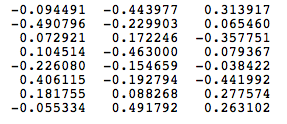
\includegraphics[width=0.4\linewidth,keepaspectratio]{word57}

$W_2$

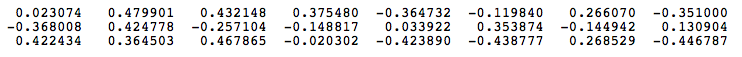
\includegraphics[width=0.8\linewidth,keepaspectratio]{word58}
\end{center}
\item Input is ``cat''' $[0 1 0 0 0 0 0 0]^T$
\item Target is ``climbed'' = $[0 0 0 1 0 0 0 0 ]t$
\end{itemize}
\end{frame}

%%%%%%%%%%%%%%%%%%%%%%%%%%%%%%%%%%%%%%%%%%%%%%%%%%%%%%%%%%%%%%%%%%%%%%%%%%%%%%%%%
\begin{frame}[fragile]\frametitle{CBOW (Continuous Bag of words)}
\begin{itemize}
\item Output at the hidden layer neurons can be computed as: $H^t = X^tW_1 = [-0.490796, -0.229903, 0.065460]$
\item Similarly for hidden to output layer: $H^tW_2$ = {\small[ 0.100934,  -0.309331,  -0.122361,  -0.151399,   0.143463,  -0.051262,  -0.079686,   0.112928]}
\item Since the goal is produce probabilities for words in the output layer, softmax is used
\item Thus, the probabilities for eight words in the corpus are:{\small 0.143073,   0.094925,   0.114441,   0.111166,   0.149289,   0.122874,   0.119431,   0.144800}
\item Error is by subtracting probability vector from the target vector.
\item Once the error is known, the weights in the matrices $W_2$ and $W_1$ can be updated using backpropagation.
\end{itemize}
\end{frame}


%%%%%%%%%%%%%%%%%%%%%%%%%%%%%%%%%%%%%%%%%%%%%%%%%%%%%%%%%%%%%%%%%%%%%%%%%%%%%%%%%
\begin{frame}[fragile]\frametitle{CBOW (Continuous Bag of words)}
\begin{itemize}
\item Given C input word vectors, the activation function for the hidden layer h amounts to simply summing the corresponding `hot' rows in W1, and dividing by C to take their average.
\item This implies that the link (activation) function of the hidden layer units is simply linear (i.e., directly passing its weighted sum of inputs to the next layer). 
\item From the hidden layer to the output layer, the second weight matrix W2 can be used to compute a score for each word in the vocabulary, and softmax can be used to obtain the posterior distribution of words.
\end{itemize}
\end{frame}

%%%%%%%%%%%%%%%%%%%%%%%%%%%%%%%%%%%%%%%%%%%%%%%%%%%%%%%%%%%%%%%%%%%%%%%%%%%%%%%%%
\begin{frame}[fragile]\frametitle{CBOW (Continuous Bag of words)}
\begin{center}
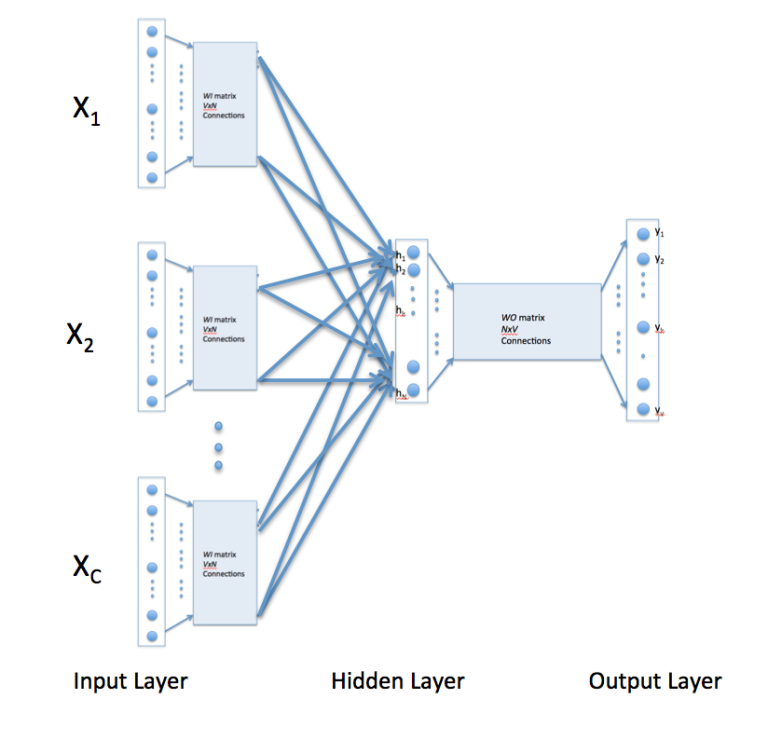
\includegraphics[width=0.6\linewidth,keepaspectratio]{word55}
\end{center}
\end{frame}

%%%%%%%%%%%%%%%%%%%%%%%%%%%%%%%%%%%%%%%%%%%%%%%%%%%%%%%%%%%%%%%%%%%%%%%%%%%%%%%%%
\begin{frame}[fragile]\frametitle{CBOW (Continuous Bag of words)}
\begin{itemize}
\item The input is multiplied by the input-hidden weights and called hidden activation. 
\item The hidden input gets multiplied by hidden- output weights and output is calculated.
\item Error between output and target is calculated and propagated back to re-adjust the weights.
\end{itemize}
\begin{center}
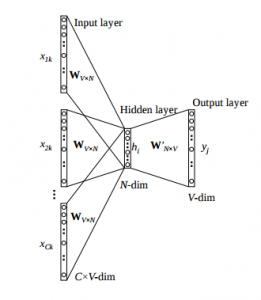
\includegraphics[width=0.3\linewidth,keepaspectratio]{word36}
\end{center}
\end{frame}

%%%%%%%%%%%%%%%%%%%%%%%%%%%%%%%%%%%%%%%%%%%%%%%%%%%%%%%%%%%%%%%%%%%%%%%%%%%%%%%%%
\begin{frame}[fragile]\frametitle{CBOW}
Advantages of CBOW:
\begin{itemize}
\item  Being probabilistic is nature, it is supposed to perform superior to deterministic methods(generally).
\item      It is low on memory. It does not need to have huge RAM requirements like that of co-occurrence matrix where it needs to store three huge matrices.
\end{itemize}
Disadvantages  of CBOW:
\begin{itemize}
\item  CBOW takes the average of the context of a word (as seen above in calculation of hidden activation). For example, Apple can be both a fruit and a company but CBOW takes an average of both the contexts and places it in between a cluster for fruits and companies.
\item  Training a CBOW from scratch can take forever if not properly optimized.
\end{itemize}
\end{frame}


%%%%%%%%%%%%%%%%%%%%%%%%%%%%%%%%%%%%%%%%%%%%%%%%%%%%%%%%%%%%%%%%%%%%%%%%%%%%%%%%%%
\begin{frame}[fragile]\frametitle{Word2Vec: Skip-Gram}
\begin{center}
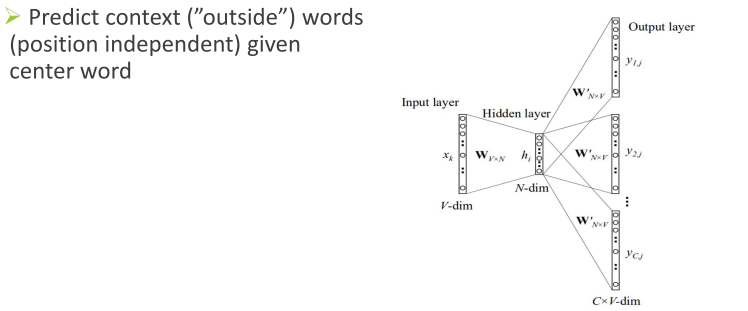
\includegraphics[width=\linewidth,keepaspectratio]{emb15}
\end{center}

{\tiny (Ref: Word Embeddings - Elena Voita, Yandex Research)}
\end{frame}


%%%%%%%%%%%%%%%%%%%%%%%%%%%%%%%%%%%%%%%%%%%%%%%%%%%%%%%%%%%%%%%%%%%%%%%%%%%%%%%%%
\begin{frame}[fragile]\frametitle{Skip-Gram Model}
\begin{itemize}
\item Skip-gram follows the same topology as of CBOW. 
\item It just flips CBOW's architecture on its head. The aim of skip-gram is to predict the context given a word. 
\item C=``Hey, this is sample corpus using only one context word.''
\end{itemize}
\begin{center}
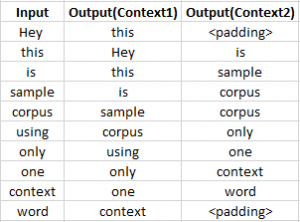
\includegraphics[width=0.6\linewidth,keepaspectratio]{word37}
\end{center}
\end{frame}

%%%%%%%%%%%%%%%%%%%%%%%%%%%%%%%%%%%%%%%%%%%%%%%%%%%%%%%%%%%%%%%%%%%%%%%%%%%%%%%%%
\begin{frame}[fragile]\frametitle{Skip-Gram Model}
\begin{itemize}
\item Since context window is of 1 on both the sides, there will be ``two'' one hot encoded target variables and ``two'' corresponding outputs as can be seen by the blue section in the image.
\item Two separate errors are calculated with respect to the two target variables and the two error vectors obtained are added element-wise to obtain a final error vector which is propagated back to update the weights.
\item The weights between the input and the hidden layer are taken as the word vector representation after training.
\end{itemize}
\end{frame}

%%%%%%%%%%%%%%%%%%%%%%%%%%%%%%%%%%%%%%%%%%%%%%%%%%%%%%%%%%%%%%%%%%%%%%%%%%%%%%%%%
\begin{frame}[fragile]\frametitle{Skip-Gram Model}
\begin{itemize}
\item Constructed with the focus word as the single input vector, and 
\item the target context words are now at the output layer
\end{itemize}
\begin{center}
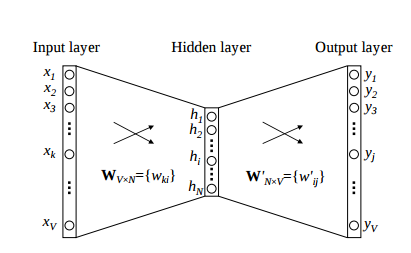
\includegraphics[width=0.8\linewidth,keepaspectratio]{word35}
\end{center}

\end{frame}


%%%%%%%%%%%%%%%%%%%%%%%%%%%%%%%%%%%%%%%%%%%%%%%%%%%%%%%%%%%%%%%%%%%%%%%%%%%%%%%%%
\begin{frame}[fragile]\frametitle{Skip-Gram Model}

\begin{center}
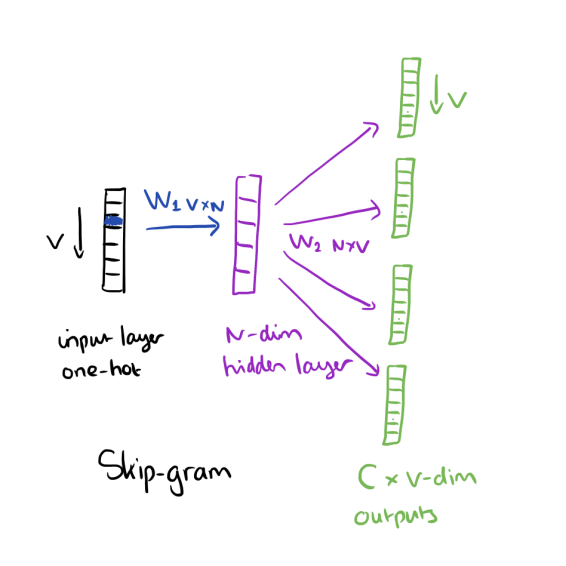
\includegraphics[width=0.5\linewidth,keepaspectratio]{word51}
\end{center}
\begin{itemize}
\item $V^T(1xv) \times W_1(vxN) = Hidden(1xN)$
\item $Hidden(1xN)  \times W_2(Nxv) = Output(1xv)  \quad  C \quad times$
\end{itemize}
\end{frame}



%%%%%%%%%%%%%%%%%%%%%%%%%%%%%%%%%%%%%%%%%%%%%%%%%%%%%%%%%%%%%%%%%%%%%%%%%%%%%%%%%
\begin{frame}[fragile]\frametitle{Skip-Gram Model}
\begin{itemize}
\item At the output layer, we now output C multinomial distributions instead of just one. 
\item The training objective is to minimize the summed prediction error across all context words in the output layer. 
\end{itemize}
\end{frame}

%%%%%%%%%%%%%%%%%%%%%%%%%%%%%%%%%%%%%%%%%%%%%%%%%%%%%%%%%%%%%%%%%%%%%%%%%%%%%%%%%%
\begin{frame}[fragile]\frametitle{Skip-Gram Model}
Context words=2, V= 10, N=4
\begin{itemize}
\item Input one-hot encoded vector.
\item  Weight matrix between the hidden layer and the output layer.
\item Matrix multiplication of hidden activation and the hidden output weights. There will be two rows calculated for two target(context) words.
\item Each output is converted into its softmax probabilities
\item Error is calculated for all output
\end{itemize}
\end{frame}

%%%%%%%%%%%%%%%%%%%%%%%%%%%%%%%%%%%%%%%%%%%%%%%%%%%%%%%%%%%%%%%%%%%%%%%%%%%%%%%%%
\begin{frame}[fragile]\frametitle{Skip-Gram Model}
Advantages of Skip-Gram Model
\begin{itemize}
\item Skip-gram model can capture two semantics for a single word. i.e it will have two vector representations of Apple. One for the company and other for the fruit.
\item     Skip-gram with negative sub-sampling outperforms every other method generally.
\end{itemize}
Disadvantages  of  Skip-Gram Model:
\begin{itemize}
\item Very vulnerable, and not a robust concept
\item Can take a long time to train
\item Non-uniform results
\item Hard to understand 
\end{itemize}
\end{frame}


%%%%%%%%%%%%%%%%%%%%%%%%%%%%%%%%%%%%%%%%%%%%%%%%%%%%%%%%%%%%%%%%%%%%%%%%%%%%%%%%%%
\begin{frame}[fragile]\frametitle{Skip-Gram Model}
\begin{itemize}
\item Skip- Gram maximizes the log - likelihood:
\begin{center}
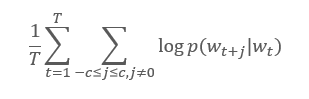
\includegraphics[width=0.4\linewidth,keepaspectratio]{word27}
\end{center}
\item Where:
\begin{itemize}
\item T - \# of words in the corpus.
\item c - unidirectional window size of the context.
\end{itemize}
\end{itemize}
\end{frame}
%%%%%%%%%%%%%%%%%%%%%%%%%%%%%%%%%%%%%%%%%%%%%%%%%%%%%%%%%%%%%%%%%%%%%%%%%%%%%%%%%
\begin{frame}[fragile]\frametitle{Skip-Gram Model}
\begin{itemize}
\item Corpus: ''If a dog chews shoes, whose shoes does he choose?''
\begin{center}
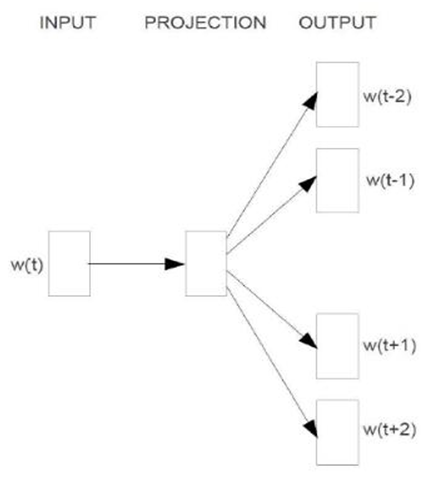
\includegraphics[width=0.4\linewidth,keepaspectratio]{word28}
\end{center}
\item Where:
\begin{itemize}
\item Input word: shoes
\item Window size: 2.
\end{itemize}
\end{itemize}
\end{frame}



%%%%%%%%%%%%%%%%%%%%%%%%%%%%%%%%%%%%%%%%%%%%%%%%%%%%%%%%%%%%%%%%%%%%%%%%%%%%%%%%%%
\begin{frame}[fragile]\frametitle{Word2Vec}
Word2vec  (Google): a distributed representation of a word is used and not sparse like One-Hot.
\begin{center}
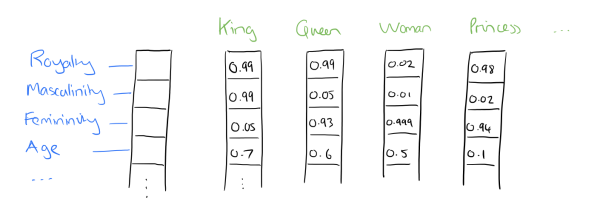
\includegraphics[width=0.8\linewidth,keepaspectratio]{word41}
\end{center}
Represent in some abstract way the `meaning' of a word.

\end{frame}

%%%%%%%%%%%%%%%%%%%%%%%%%%%%%%%%%%%%%%%%%%%%%%%%%%%%%%%%%%%%%%%%%%%%%%%%%%%%%%%%%%
\begin{frame}[fragile]\frametitle{Word Distributed Representation - Word2Vec}
\begin{itemize}
\item All vector cells participate in representing each word.
\item Words are represented by real valued dense vectors of significantly smaller dimensions (e.g. 100 - 1000).
\item  Intuition: consider each vector cell as a representative of some feature.
\begin{center}
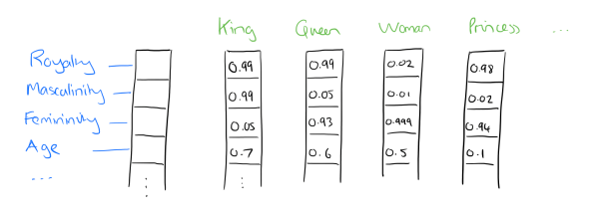
\includegraphics[width=\linewidth,keepaspectratio]{word24}
\end{center}
\end{itemize}
\end{frame}




%%%%%%%%%%%%%%%%%%%%%%%%%%%%%%%%%%%%%%%%%%%%%%%%%%%%%%%%%%%%%%%%%%%%%%%%%%%%%%%%%%
\begin{frame}[fragile]\frametitle{Word Representations Comparison}

\adjustbox{valign=t}{
\begin{minipage}{0.45\linewidth}
Traditional Method  - Bag of Words Model

\begin{itemize}
\item Uses one hot encoding
\item Each word in the vocabulary is represented by one bit position in a HUGE vector.
\item For example, with a vocabulary of 10000 words, and ''Hello'' is the 4th word in the dictionary:  \lstinline|0 0 0 1 0 0  . . . . . . . 0 0 0 0 |
\item Context information is not utilized
\end{itemize}
\end{minipage}
}
\hfill
\adjustbox{valign=t}{
\begin{minipage}{0.45\linewidth}
Modern - Word Vectors

\begin{itemize}
\item Stores each word in as a point in space, represented by a vector of fixed number of dimensions (generally 300)
\item Unsupervised, built just by reading huge corpus
\item For example, ''Hello'' might be represented as :  \lstinline| [0.4, -0.11, 0.55, 0.3 . . . 0.1, 0.02]|
\item Context information is utilized
\end{itemize}
\end{minipage}
}
\end{frame}



%%%%%%%%%%%%%%%%%%%%%%%%%%%%%%%%%%%%%%%%%%%%%%%%%%%%%%%%%%%%%%%%%%%%%%%%%%%%%%%%%%
\begin{frame}[fragile]\frametitle{The Power of Word2Vecs}

\begin{itemize}
\item They provide a fresh perspective to ALL  problems in NLP, and not just solve one problem.
\item Technological Improvement
\item Rise of deep learning since 2006 (Big Data + GPUs  + Work done by Andrew Ng, Yoshua Bengio, Yann Lecun and Geoff Hinton)
\item Application of Deep Learning to NLP - led by Yoshua Bengio,  Christopher Manning, Richard Socher, Tomas Mikalov
\item The need for unsupervised learning . (Supervised learning tends to be excessively dependent on hand-labeled data and often does not scale)
\end{itemize}
\end{frame}


%%%%%%%%%%%%%%%%%%%%%%%%%%%%%%%%%%%%%%%%%%%%%%%%%%%%%%%%%%%%%%%%%%%%%%%%%%%%%%%%%%
\begin{frame}[fragile]\frametitle{Examples}
Vectors for King, Man, Queen, \& Woman:
\begin{center}
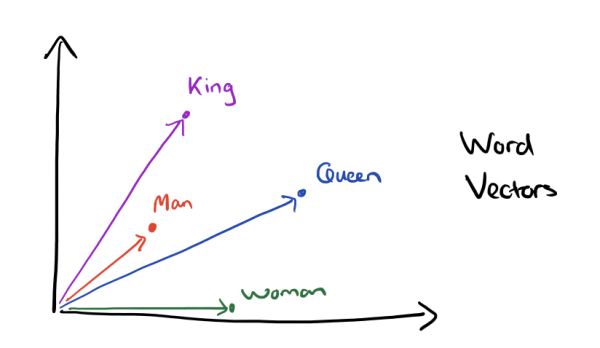
\includegraphics[width=0.5\linewidth,keepaspectratio]{word42}
\end{center}


\begin{center}
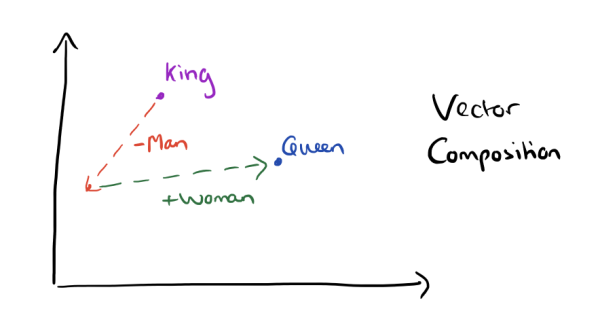
\includegraphics[width=0.5\linewidth,keepaspectratio]{word44}
\end{center}

\end{frame}

%%%%%%%%%%%%%%%%%%%%%%%%%%%%%%%%%%%%%%%%%%%%%%%%%%%%%%%%%%%%%%%%%%%%%%%%%%%%%%%%%%
\begin{frame}[fragile]\frametitle{Examples}
Gender relation:
\begin{center}
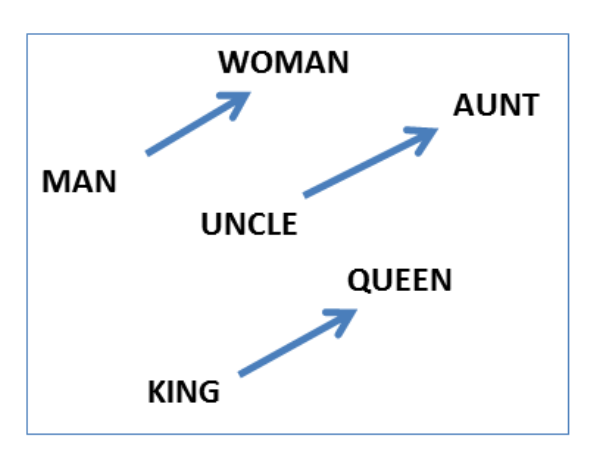
\includegraphics[width=0.35\linewidth,keepaspectratio]{word45}
\end{center}
Plural relation:

\begin{center}
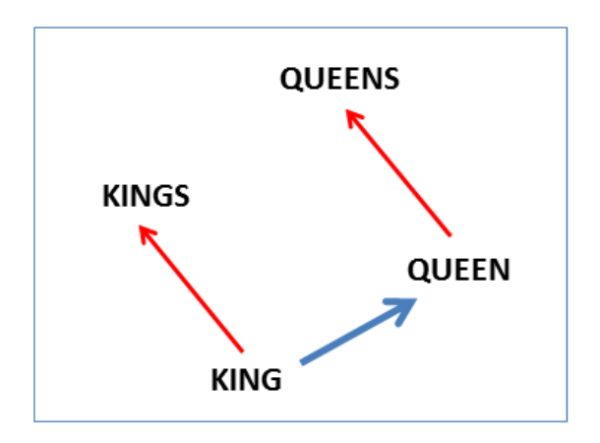
\includegraphics[width=0.35\linewidth,keepaspectratio]{word46}
\end{center}

\end{frame}


%%%%%%%%%%%%%%%%%%%%%%%%%%%%%%%%%%%%%%%%%%%%%%%%%%%%%%%%%%%%%%%%%%%%%%%%%%%%%%%%%%
\begin{frame}[fragile]\frametitle{Examples}
Word pair relationships:
\begin{center}
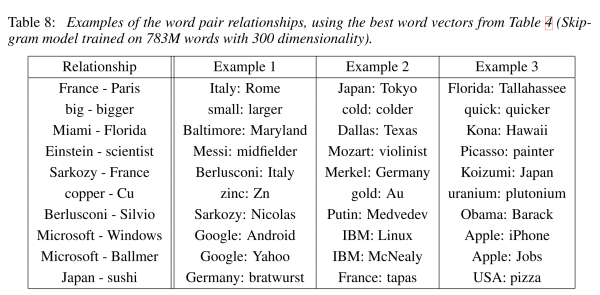
\includegraphics[width=0.4\linewidth,keepaspectratio]{word47}
\end{center}
Country-capital city relationship:

\begin{center}
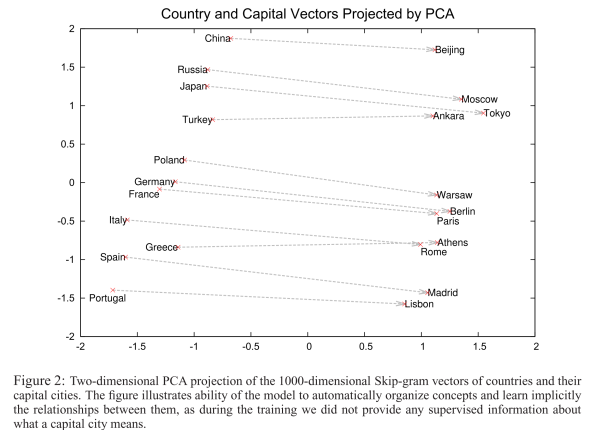
\includegraphics[width=0.4\linewidth,keepaspectratio]{word48}
\end{center}

\end{frame}

%%%%%%%%%%%%%%%%%%%%%%%%%%%%%%%%%%%%%%%%%%%%%%%%%%%%%%%%%%%%%%%%%%%%%%%%%%%%%%%%%%
\begin{frame}[fragile]\frametitle{What if \ldots}
We want to use subword
information?
\end{frame}

%%%%%%%%%%%%%%%%%%%%%%%%%%%%%%%%%%%%%%%%%%%%%%%%%%%%%%%%%%%%%%%%%%%%%%%%%%%%%%%%%%
\begin{frame}[fragile]\frametitle{FastText}
Adding subword information
\begin{itemize}
\item  Model: SG-NS (skip-gram with negative sampling)
\item Change the way word vectors are formed
\item  each word represented as a bag of character 
n-gram: eg ``where'' : "wh","whe","her","ere","re"
\item  associate a vector representation to each n-
gram 
\item  represent a word by the sum of the vector 
representations of its n-grams
\end{itemize}

{\tiny (Ref: Bojanovsky et al, TACL 2017 http://aclweb.org/anthology/Q17-1010)}

\end{frame}

%%%%%%%%%%%%%%%%%%%%%%%%%%%%%%%%%%%%%%%%%%%%%%%%%%%%%%%%%%%%%%%%%%%%%%%%%%%%%%%%%%
\begin{frame}[fragile]\frametitle{What if \ldots}
We abstract the skip-gram 
model to the sentence level?
\end{frame}

%%%%%%%%%%%%%%%%%%%%%%%%%%%%%%%%%%%%%%%%%%%%%%%%%%%%%%%%%%%%%%%%%%%%%%%%%%%%%%%%%%
\begin{frame}[fragile]\frametitle{Sentence Embedding}

\begin{itemize}
\item  Before: use a word to predict its 
surrounding context
\item Now: encode a sentence to predict 
the sentences around it 
\end{itemize}

{\tiny (Ref: Kiros et al., NIPS 2015 https://papers.nips.cc/paper/5950-skip-thought-vectors.pdf)}
\end{frame}

%%%%%%%%%%%%%%%%%%%%%%%%%%%%%%%%%%%%%%%%%%%%%%%%%%%%%%%%%%%%%%%%%%%%%%%%%%%%%%%%%%
\begin{frame}[fragile]\frametitle{Latest embeddings}

\begin{itemize}
\item  The year 2018 has been an inflection point for machine learning models in NLP 
\item It’s been referred to as NLP’s ImageNet moment,
\end{itemize}

\begin{center}
\includegraphics[width=0.7\linewidth,keepaspectratio]{emb16}
\end{center}

{\tiny (Ref: The Illustrated BERT, ELMo, and co. (How NLP Cracked Transfer Learning) -Jay Alammar )}
\end{frame}

%%%%%%%%%%%%%%%%%%%%%%%%%%%%%%%%%%%%%%%%%%%%%%%%%%%%%%%%%%%%%%%%%%%%%%%%%%%%%%%%%%
\begin{frame}[fragile]\frametitle{ELMo: Context Matters}
\begin{itemize}
\item  Say, a word “stick” would be represented by a Word2Vec vector no-matter what the context was. 
\item  “stick”” has multiple meanings depending on where it’s used. 
\item Why not give it an embedding based on the context it’s used in – to both capture the word meaning in that context as well as other contextual information?”. 
\item Instead of using a fixed embedding for each word, ELMo looks at the entire sentence before assigning each word in it an embedding. It uses a bi-directional LSTM trained on a specific task to be able to create those embeddings.

\end{itemize}


{\tiny (Ref: The Illustrated BERT, ELMo, and co. (How NLP Cracked Transfer Learning) -Jay Alammar )}
\end{frame}

%%%%%%%%%%%%%%%%%%%%%%%%%%%%%%%%%%%%%%%%%%%%%%%%%%%%%%%%%%%%%%%%%%%%%%%%%%%%%%%%%%
\begin{frame}[fragile]\frametitle{ULM-FiT: Nailing down Transfer Learning in NLP}
\begin{itemize}
\item  ULM-FiT introduced methods to effectively utilize a lot of what the model learns during pre-training – more than just embeddings, and more than contextualized embeddings. ULM-FiT introduced a language model and a process to effectively fine-tune that language model for various tasks.
\item NLP finally had a way to do transfer learning probably as well as Computer Vision could
\end{itemize}


{\tiny (Ref: The Illustrated BERT, ELMo, and co. (How NLP Cracked Transfer Learning) -Jay Alammar )}
\end{frame}

%%%%%%%%%%%%%%%%%%%%%%%%%%%%%%%%%%%%%%%%%%%%%%%%%%%%%%%%%%%%%%%%%%%%%%%%%%%%%%%%%%
\begin{frame}[fragile]\frametitle{The Transformer: Going beyond LSTMs}
\begin{itemize}
\item The Encoder-Decoder structure of the transformer made it perfect for machine translation. But how would you use it for sentence classification? 
\item How would you use it to pre-train a language model that can be fine-tuned for other tasks?
\end{itemize}


{\tiny (Ref: The Illustrated BERT, ELMo, and co. (How NLP Cracked Transfer Learning) -Jay Alammar )}
\end{frame}

%%%%%%%%%%%%%%%%%%%%%%%%%%%%%%%%%%%%%%%%%%%%%%%%%%%%%%%%%%%%%%%%%%%%%%%%%%%%%%%%%%
\begin{frame}[fragile]\frametitle{OpenAI Transformer}
Pre-training a Transformer Decoder for Language Modeling 
\begin{itemize}
\item It turns out we don’t need an entire Transformer to adopt transfer learning and a fine-tunable language model for NLP tasks. 
\item We can do with just the decoder of the transformer. The decoder is a good choice because it’s a natural choice for language modeling (predicting the next word) since it’s built to mask future tokens – a valuable feature when it’s generating a translation word by word.
\item Now that the OpenAI transformer is pre-trained and its layers have been tuned to reasonably handle language, we can start using it for downstream tasks.
\end{itemize}


{\tiny (Ref: The Illustrated BERT, ELMo, and co. (How NLP Cracked Transfer Learning) -Jay Alammar )}
\end{frame}

%%%%%%%%%%%%%%%%%%%%%%%%%%%%%%%%%%%%%%%%%%%%%%%%%%%%%%%%%%%%%%%%%%%%%%%%%%%%%%%%%%
\begin{frame}[fragile]\frametitle{BERT: From Decoders to Encoders}
\begin{itemize}
\item The openAI transformer gave us a fine-tunable pre-trained model based on the Transformer. But something went missing in this transition from LSTMs to Transformers. 
\item ELMo’s language model was bi-directional, but the openAI transformer only trains a forward language model. 
\item Could we build a transformer-based model whose language model looks both forward and backwards (in the technical jargon – “is conditioned on both left and right context”)?
\item 
“Hold my beer”, said R-rated BERT. Everybody knows bidirectional conditioning would allow each word to indirectly see itself in a multi-layered context.” “We’ll use masks”, said BERT confidently.
\end{itemize}


{\tiny (Ref: The Illustrated BERT, ELMo, and co. (How NLP Cracked Transfer Learning) -Jay Alammar )}
\end{frame}


%%%%%%%%%%%%%%%%%%%%%%%%%%%%%%%%%%%%%%%%%%%%%%%%%%%%%%%%%%%%%%%%%%%%%%%%%%%%%%%%%%
\begin{frame}[fragile]\frametitle{BERT}
So, BERT builds on top of a number of clever ideas that have been bubbling up in the NLP community recently – 
including but not limited to 
\begin{itemize}
\item  Semi-supervised Sequence Learning (by Andrew Dai and Quoc Le), 
\item  ELMo (by Matthew Peters and researchers from AI2 and UW CSE), 
\item  ULMFiT (by fast.ai founder Jeremy Howard and Sebastian Ruder), 
\item  the OpenAI transformer (by OpenAI researchers Radford, Narasimhan, Salimans, and Sutskever), and 
\item  the Transformer (Vaswani et al).
\end{itemize}

You can use the pre-trained BERT to create contextualized word embeddings

{\tiny (Ref: The Illustrated BERT, ELMo, and co. (How NLP Cracked Transfer Learning) -Jay Alammar )}
\end{frame}



%%%%%%%%%%%%%%%%%%%%%%%%%%%%%%%%%%%%%%%%%%%%%%%%%%%%%%%%%%%%%%%%%%%%%%%%%%%%%%%%%%
\begin{frame}[fragile]\frametitle{How to evaluate embeddings}
Intrinsic: evaluation on a specific/intermediate subtask
\begin{itemize}
\item  word analogies: “a is to b as c is to \underline{xxxx}?” 
\item  word similarity: correlation of the rankings
\end{itemize}
Extrinsic: evaluation on a real task
\begin{itemize}
\item  take some task (MT, NER, coreference resolution, …) or several tasks
\item   train with different pretrained word embeddings
\item  if the task quality is better -> win!
\end{itemize}
\end{frame}


%%%%%%%%%%%%%%%%%%%%%%%%%%%%%%%%%%%%%%%%%%%%%%%%%%%%%%%%%%%%%%%%%%%%%%%%%%%%%%%%%%
\begin{frame}[fragile]\frametitle{}

\begin{center}
{\Large Applications of Word Vectors}
\end{center}
\end{frame}




%%%%%%%%%%%%%%%%%%%%%%%%%%%%%%%%%%%%%%%%%%%%%%%%%%%%%%%%%%%%%%%%%%%%%%%%%%%%%%%%%%
\begin{frame}[fragile]\frametitle{Applications of Word Vectors}
Word Similarity:

\begin{itemize}
\item Classic Methods :  Edit Distance, WordNet, Porter's Stemmer, Lemmatization using dictionaries
\item Easily identifies similar words and synonyms since they occur in similar contexts
\item Stemming (thought $\rightarrow$ think) 
\item Inflections, Tense forms
\item eg. Think, thought, ponder, pondering,
\item eg. Plane, Aircraft, Flight
\end{itemize}
\end{frame}


%%%%%%%%%%%%%%%%%%%%%%%%%%%%%%%%%%%%%%%%%%%%%%%%%%%%%%%%%%%%%%%%%%%%%%%%%%%%%%%%%%
\begin{frame}[fragile]\frametitle{Applications of Word Vectors}
Machine Translation:

\begin{itemize}
\item Classic Methods :  Rule-based machine translation, morphological transformation
\begin{center}
\includegraphics[width=0.6\linewidth,keepaspectratio]{word13}
\end{center}
\end{itemize}
\end{frame}

%%%%%%%%%%%%%%%%%%%%%%%%%%%%%%%%%%%%%%%%%%%%%%%%%%%%%%%%%%%%%%%%%%%%%%%%%%%%%%%%%%
\begin{frame}[fragile]\frametitle{Applications of Word Vectors}
Part-of-Speech and Named Entity Recognition:

\begin{itemize}
\item Classic Methods :  Sequential Models (MEMM , Conditional Random Fields),  Logistic Regression
\begin{center}
\includegraphics[width=0.8\linewidth,keepaspectratio]{word10}
\end{center}
\end{itemize}
\end{frame}
%
%%%%%%%%%%%%%%%%%%%%%%%%%%%%%%%%%%%%%%%%%%%%%%%%%%%%%%%%%%%%%%%%%%%%%%%%%%%%%%%%%%%
%\begin{frame}[fragile]\frametitle{Applications of Word Vectors}
%Relation Extraction:
%
%\begin{itemize}
%\item Classic Methods : OpenIE, Linear programing models, Bootstrapping
%\begin{center}
%\includegraphics[width=0.8\linewidth,keepaspectratio]{word11}
%\end{center}
%\end{itemize}
%\end{frame}

%%%%%%%%%%%%%%%%%%%%%%%%%%%%%%%%%%%%%%%%%%%%%%%%%%%%%%%%%%%%%%%%%%%%%%%%%%%%%%%%%%
\begin{frame}[fragile]\frametitle{Applications of Word Vectors}
Sentiment Analysis:
\begin{itemize}
\item Classic Methods : Naive Bayes, Random Forests/SVM
\item Classifying sentences as positive and negative
\item Building sentiment lexicons using seed sentiment sets
\item No need for classifiers, we can just use cosine distances to compare unseen reviews to known reviews.

\begin{center}
\includegraphics[width=0.7\linewidth,keepaspectratio]{word15}
\end{center}
\end{itemize}
\end{frame}

%%%%%%%%%%%%%%%%%%%%%%%%%%%%%%%%%%%%%%%%%%%%%%%%%%%%%%%%%%%%%%%%%%%%%%%%%%%%%%%%%%
\begin{frame}[fragile]\frametitle{Applications of Word Vectors}
Sentiment Analysis:
\begin{itemize}
\item Co-reference Resolution: Chaining entity mentions across multiple documents  - can we find and unify the multiple contexts in which mentions occurs?
\item Clustering: Words in the same class naturally occur in similar contexts,  and this feature vector can directly be used with any conventional clustering algorithms (K-Means, agglomerative, etc). Human doesn't have to waste time hand-picking useful word features to cluster on.
\item Semantic Analysis of Documents: Build word distributions for various topics, etc.

\end{itemize}
\end{frame}
%%%%%%%%%%%%%%%%%%%%%%%%%%%%%%%%%%%%%%%%%%%%%%%%%%%%%%%%%%%%%%%%%%%%%%%%%%%%%%%%%%%
%\begin{frame}[fragile]\frametitle{Weakness of Word Embedding}
%\begin{itemize}
%\item Very vulnerable, and not a robust concept
%\item Can take a long time to train
%\item Non-uniform results
%\item Hard to understand and visualize
%\end{itemize}
%\end{frame}